\documentclass[11pt, a4paper]{article}

\usepackage[utf8]{inputenc}
\usepackage{graphicx}
\graphicspath{ {images/} }
\usepackage{mathtools}
\usepackage{amssymb}
\usepackage{amsmath}
\usepackage[ngerman,english]{babel}
\usepackage{cite}
\usepackage{bibgerm}
\usepackage{fullpage}
\usepackage[top=1.5cm,bottom=1.5cm,left=3.5cm,right=2.5cm,headsep=1.5cm,includeheadfoot]{geometry}
\usepackage{tabularx}
\usepackage{caption}
\usepackage{subcaption}
\usepackage{eurosym}
\usepackage{enumitem}
\usepackage{multicol}
\usepackage{tikz}
\usepackage{tkz-euclide}
\usepackage{pgfplots}
\usepackage{pdflscape}
\usepackage{acronym}
\usepackage{blindtext}
\usepackage{ifthen}
\usepackage{setspace}
\usepackage{cancel}
\usepackage{color}
\usepackage{listings}
\usepackage{comment}
\usepackage{xcolor}
\usepackage{colortbl}
\usepackage[parfill]{parskip}
\usepackage{url}

\usepackage{fancyhdr}
\pagestyle{fancy}

\fancyhf{} % clear all
\fancyhead[L]{\leftmark}
\fancyfoot[C]{-- \thepage{} --}
%\setlength{\headheight}{15pt}
\renewcommand{\headrulewidth}{0.5pt}
\renewcommand{\footrulewidth}{0pt}
\setlength{\skip\footins}{0.7cm}

\usetikzlibrary{graphs}
\usetikzlibrary{positioning}

\onehalfspacing
\setlength\parindent{0pt}

%\everymath{\displaystyle}

\allowdisplaybreaks

\definecolor{AI-BLUE}{rgb}{0,0.57,0.87}

% Eigene Befehle
\newcommand\q[1]{\glqq{}#1\grqq{}}
\renewcommand\equiv{\Leftrightarrow}
\newcommand\vertequal[2]{\underset{\underset{#2}{\parallel}}{#1}}
\newcommand\cif{\text{if }}
\newcommand\abs[1]{\left|#1\right|}
\newcommand\norm[1]{\abs{\abs{#1}}}
\newcommand\diff[1]{\text{ d#1}}
\newcommand\av[1]{\left\langle#1\right\rangle}
\newcommand\ev[1]{\mathbb{E}\left(#1\right)}
\newcommand\br[1]{\left(#1\right)}
\newcommand\ubr[2]{\underbrace{#1}_{#2}}
\newcommand\quer[1]{\overline{#1}}
\newcommand\setequal{\overset{!}{=}}
\newcommand\dint{\displaystyle \int}
\newcommand\dsum{\displaystyle \sum}
\newcommand\dprod{\displaystyle \prod}
\newcommand\closedInt[2]{\left[#1,#2\right]}
\newcommand{\checkbox}{\Large \Square \normalsize \hspace{0.4cm}}

\newcommand\myref[1]{\ref{#1} (S. \pageref{#1})}
\newcommand\myrefcomma[1]{\ref{#1}, S. \pageref{#1}}

\begin{document}

\thispagestyle{empty}

\setlength{\hoffset}{-0.5cm} % center title page

\lstset{
  basicstyle=\small,           % the size of the fonts that are used for the code
  breaklines=true,             % sets automatic line breaking
  captionpos=b,                % sets the caption-position to bottom
  frame=single,                % adds a frame around the code
  keepspaces=true,             % keeps spaces in text, useful for keeping indentation of code (possibly needs columns=flexible)
  numbers=right,               % where to put the line-numbers; possible values are (none, left, right)
  showspaces=false,            % show spaces everywhere adding particular underscores; it overrides 'showstringspaces'
  stepnumber=1,                % the step between two line-numbers. If it's 1, each line will be numbered
  tabsize=4,                   % sets default tabsize to 4 spaces
  xleftmargin=0.14cm		   % sets left margin
}

\begin{titlepage}
    \begin{center}
    \Large \textbf{Master's Thesis}\\
    \vspace{3cm}
    \normalsize
    Master's Thesis\\
    in the Program of Applied Computer Science\\
    at the Ruhr-University Bochum\\
    at the Institute for Neural Computation\\
    in the Summer Term 2016\\
    \vspace{3cm}
    \LARGE \textbf{A Deep Convolutional Network for Facial Landmark Estimation} \\
    \vspace{3cm}
    \normalsize
    \textbf{Author:}\\
    Schrör, Phil Yannick\\
    108 011 214 024\\
    \vspace{2cm}
    \textbf{To be handed in:}\\
    31st of October 2016\\
    \vspace{2cm}
    \textbf{Supervisors:}\\
    PD Dr. Rolf P. Würtz\\
    M.Sc. Andreas Nilkens
    \end{center}
\end{titlepage}

\newpage
\pagenumbering{arabic}
\setcounter{page}{2}

\tableofcontents

\newpage

\addcontentsline{toc}{section}{List of Acronyms}

\section*{List of Acronyms}
\markboth{LIST OF ACRONYMS}{}

%\acrodefplural{KNN}[KNN]{Künstliche Neuronale Netzwerke}

\begin{acronym}
\acro{ANN}{Artificial Neural Network}
\acro{CNN}{Convolutional Neural Network}
\acro{MUCT}{Milborrow / University of Cape Town} (Image data set)
\acro{RGB}{Red Green Blue}
\acro{SGD}{Stochastic Gradient Descent}
\end{acronym}


%\subsection*{Color legend} %TODO Remove me
%\textcolor{purple}{purple: find better synonym}

\newpage

\section{Introduction}

\acp{ANN} have proven to be very powerful tools developed and used in the field of Neural Computation. Particularly \acp{CNN} exhibit a solid performance on grafical data like images or videos. Finding patterns and hidden structures in images can be very useful in many respects, one of them is the diagnosis of diseases which influence the appearance of the human face\footnote{cf. \cite{ebgm}}. For that reason \acp{CNN} are used in the scope of this thesis to estimate the position of so called landmarks in images of human faces. While some of those landmarks are preeminent featuers like the eyes or the tip of the nose, other landmarks are less prominent points, which are harder to find.\\
Since tagging all those landmarks by hand is a tedious work, it is disireable to create an automatism, which estimates them. In order to reach this goal two different general network architectures are used and tested in many different configurations. Both kinds of network take an RGB-image of a human face as input and produce the estimated coordinates of the landmarks as output. The first approach, however, trains a complete \ac{CNN} conventionally, i.e. all the network's weights are initialized randomly and subsequently trained by the \ac{SGD} optimization method. The second approach, on the other hand, uses Gabor wavelets as weights for the first layer of the \ac{CNN}. In this kind of network only the weights of the subsequent layers are trained, while the Gabor wavelets remain unchainged throughout the whole training phase. The Gabor responses are then combined and forwarded through the subsequent layers of the network.\\
In order to compare the two approaches a \ac{CNN} with the same structure as used with the Gabor wavelets has been trained completly. \dots\\%TODO Elaborate this
Testing the different networks has shown that \dots%TODO Write more!

% Completely trained network with the dimensions of the gabor network
% Hint some of the results

\newpage

\section{Neural Networks}

\subsection{Artificial Neural Networks}

\subsection{Convolutional Neural Networks}

\newpage

\section{Data}

Training and testing a \ac{CNN} requires an appropriate data set with a sufficiently large number of training and test examples. Daniel Nouri uses the data set from the \emph{Facial Keypoints Detection} challenge on the machine learning website Kaggle\footnote{cf. \cite{kaggle}} in his inspiring tutorial \emph{Using convolutional neural nets to detect facial keypoints}\footnote{cf. \cite{nouri-tutorial}}. This dataset provides a reasonable amount of landmarks, however, it does not provide all landmarks for all faces. To avoid too much data organisation overhead it was used the \ac{MUCT} data set\footnote{cf. \cite{muct}} instead, which exhibits a simpler structure and provides not only all kaggle landmarks but even more for each depicted person.

\subsection{Kaggle}

Since the first experiments done in the scope of this thesis were inspired by the tutorial by Daniel Nouri named above, it was initially worked with the same data set, which was used there. The contemplated data set is taken from the \emph{Facial Keypoints Detection} challenge on Kaggle and contains 7049 training images as well as 1783 test images with a resolution of $96 \times 96$ pixels. All images are provided as gray value images within the range $[0,255]$.\\
There are 15 different landmarks (called keypoints on Kaggle), each of which consists of two scalar values $(x,y)$, which represent the horizontal and vertical position of the corresponding feature in the image. The 15 landmarks are:
\begin{multicols}{2}
	\begin{itemize}[itemsep=-2ex]
		\item Left eye center
		\item Right eye center
		\item Left eye inner corner
		\item Left eye outer corner
		\item Right eye inner corner
		\item Right eye outer corner
		\item Left eyebrow inner end
		\item Left eyebrow outer end
	\end{itemize}
\columnbreak
	\begin{itemize}[itemsep=-2ex]
		\item Right eyebrow inner end
		\item Right eyebrow outer end
		\item Nose tip
		\item Mouth left corner
		\item Mouth right corner
		\item Mouth center top lip
		\item Mouth center bottom lip
	\end{itemize}
	\vphantom{}
\end{multicols}
As already mentioned, not all landmarks exist for all images. In fact, for almost all landmarks exists an individiual number of images containing them. This leads to problems, because a \ac{CNN} expects a fixed number of inputs and a produces a fixed number of outputs. It is difficult to develope a mechanism, which checks for each input image how many landmarks are actually given and then includes only these landmarks into the calculation of the error function. Since using this data set would have required a comparatively high organization effort and since the resolution of $96 \times 96$ is rather small, another data set with a larger resolution of the raw images was used.

\subsection{MUCT Face Database}

The \acf{MUCT} face database was created by Stephen Millborrow, John Morkel and Fred Nicolls in December 2008 at the University Of Cape Town.\footnote{cf. \cite{muct}} It contains 3755 faces with 76 manually set landmarks, including all Kaggle landmarks presented above. As shown in figure \ref{fig:muctfaces}, it provides a broad spectrum of faces from people of different age, gender and ethnicity. Furthermore, many different lighting settings have been used in order to increase the diversity of the pictures.

\begin{figure}[htbp]
	\centering
	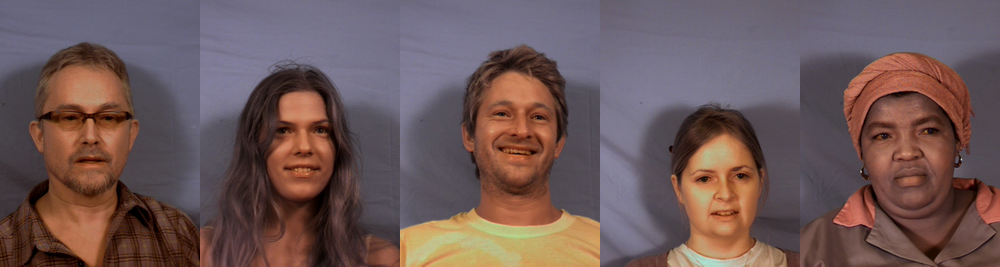
\includegraphics[width=\textwidth]{muct_faces.png}
	\caption{Five faces from the MUCT Face Database}
	\label{fig:muctfaces}
\end{figure}

Since images given in real applications are often not taken from a perfectly frontal perspective on the face, the creators of the data set provide images taken from five different angles, which are shown in figure \ref{fig:muctangles}. Disregarding some software induced delays, all five images were taken simultaneously in order to guarantee that the person does not move between two photo shots. Whereas two of the images show the right side of the person's face, images of the left side were not taken, because approximations of these images can be easily obtained by mirroring.

\begin{figure}[htbp]
	\centering
	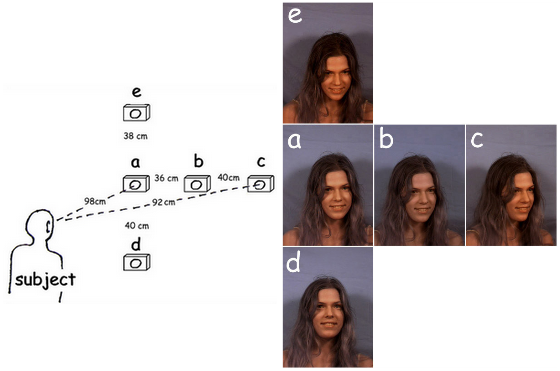
\includegraphics[width=0.77\textwidth]{muct_perspectives.png}
	\caption[MUCT Different Perspectives]{MUCT Different Perspectives\footnotemark}
	\label{fig:muctangles}
\end{figure}
\footnotetext{Both illustrations were taken from the \cite{muct} paper}

There is only one real disadvantage of the \ac{MUCT} data set compared to the Kaggle data set, i.e. the smaller total number of images -- 3755 on \ac{MUCT} instead of 8832 on Kaggle. In fact, using the \ac{MUCT} data set has a lot of advantages. The first one is the larger resolution: the \ac{MUCT} images are made available in a resolution of $480 \times 640$ pixels, whereas the Kaggle images have a resolution of only $96 \times 96$ pixels. The lager resolution allows for a model, which works more precisely with regard to rather subtle or fine landmarks. Another advantage is the accessibility of colour information, which may be useful to produce a reasonable predicition at the cost of a longer program execution time.\\
Another expedient property of the \ac{MUCT} data set is its well-structuredness. The file names contain all relevant information about the corresponding image, because all of them follow the pattern: \texttt{i\{personID\}\{lighting set\}\{camera view\}-\{gender\}\{(no) glasses\}}. The first \texttt{i}mage of the data set has the file name \texttt{i000qa-fn.jpg}, so the person has the ID \texttt{000}, lighting setting \texttt{q} was used, the photo was shot from angle \texttt{a}, the person is \texttt{f}emale and does \texttt{n}ot wear glasses.\\
This naming system is highly valuable, because selecting only a certain subset of the images is simplified a lot, because it is sufficient to check their filename for a specific character at the corresponding position. This is important, because also the \ac{MUCT} data set does not provide all landmarks for all images, but it does so in a much more organized way. It occurs only for the camera views \texttt{b} and \texttt{c} that some landmarks may not be given, because some of them are not visible due to the perspective on the face. For example the end of the person's left eyebrow ist often not visible.\\
Since \acp{ANN} usually require a fixed input size and a fixed output size, all images taken from camera view \texttt{b} and \texttt{c} were omitted and not used at all. For that reason the total number of images decreases to 2257, which were divided randomly in 1752 training images and 502 test images. In order to increase the generalization capability of the network, no person was assigned to both training set and test set. Hence, the test images presented to the network always showed persons unknown to the network.

\newpage

\section{Network Architectures}

\subsection{Thoroughly trained CNN}

\subsection{Using Gabor Wavelets}

\newpage

\section{Results}

\subsection{Thoroughly trained CNN}

\begin{itemize}
\item Gridsearch
\item Momentum (bad!?)
\item Decay (bad, too!?)
\end{itemize}

\subsection{Using Gabor Wavelets}

\begin{itemize}
\item Small resolution, absolute value
\item Small resolution, arctan2
\item Larger resolution, absolute value
\item Larger resolution, arctan2
\end{itemize}

\subsection{Confrontation of both Approaches}

Gabor approach probably better

\newpage

\section{Conclusion}

\newpage

\begin{appendix}
	\section{Implementation}
	
	Theano\footnote{cf. \cite{theano}} was used.
	
\end{appendix}

\newpage

\addcontentsline{toc}{section}{List of Figures}
\listoffigures

\newpage

\addcontentsline{toc}{section}{References}
%\section*{References} %TODO Remove me
\bibliography{ref}{}
\bibliographystyle{alpha}
%http://www.cs.toronto.edu/$\sim$tijmen/csc321/slides/lecture\_slides\_lec6.pdf\\
%http://cs231n.github.io/neural-networks-3/

\newpage

\thispagestyle{empty}

\begin{center}
\subsection*{Erklärung / Declaration}
\end{center}
\vspace{0.5cm}
Ich erkläre, dass das Thema dieser Arbeit nicht identisch ist mit dem Thema einer von mir bereits für eine andere Prüfung eingereichten Arbeit.\\
Ich erkläre weiterhin, dass ich die Arbeit nicht bereits an einer anderen Hochschule zur Erlangung eines akademischen Grades eingereicht habe.

\vspace{0.8cm}
Ich versichere, dass ich die Arbeit selbstständig verfasst und keine anderen als die angegebenen Quellen benutzt habe. Die Stellen der Arbeit, die anderen Werken dem Wortlaut oder dem Sinn nach entnommen sind, habe ich unter Angabe der Quellen der Entlehnung kenntlich gemacht. Dies gilt sinngemäß auch für gelieferte Zeichnungen, Skizzen, bildliche Darstellungen und dergleichen.

\vspace{2cm}
I declare that the topic of this thesis is not identical to the topic of another thesis written by me for another examination. Furthermore I declare that I did not submit this thesis to another university to obtain an academic degree.

\vspace{0.8cm}
I assure that I composed this thesis thoroughly on my own without using other sources than the denoted ones. Those fragments of this thesis, which are taken literally or figuratively from other works, are indicated by citing their origin. This also applies to the provided drawings, sketches, illustrations and suchlike.

\vspace{1.5cm}
\rule[0.05cm]{5cm}{0.5pt} \hspace{4.5cm} \rule[0.05cm]{5cm}{0.5pt}\\
Datum / Date \hspace{7.1cm} Unterschrift / Signature

\end{document}






